\documentclass[a4paper,12pt]{article}
\usepackage{czech}
\usepackage[utf8]{inputenc}
\usepackage{a4wide}
\usepackage[dvipdfm]{graphicx}
\usepackage{graphics}
\usepackage{indentfirst}
\usepackage{fancyhdr}
\usepackage{setspace}
\usepackage{amsmath}
\usepackage{amssymb}
\usepackage{epsfig}

%%\usepackage{nopageno}
%%\usepackage{txfonts}
\usepackage[usenames]{color}

\begin{document}
\section{Úkol}
\noindent
\begin{enumerate}
    \item Změřte metodou přímou závislost odporu vlákna žárovky na proudu, který jím protéká. K měření použijte stejnosměrné napětí v rozsahu do 24 V.
    \item Změřte substituční metodou vnitřní odpor měřicích přístrojů použitých v úkolu 1. Výsledek použijte k případné korekci naměřených hodnot odporů v úkolu 1.
    \item Metodou substituční změřte závislost odporu vlákna žárovky na proudu od nejmenších proudů (0,2 mA) až do 25 mA. Porovnejte přesnost výsledků s přesností dosaženou v úkolu 1.
    \item Výsledky zpracujte graficky a diskutujte vliv měřících přístrojů.
    \item Stanovte odpor vlákna žárovky při pokojové teplotě. K extrapolaci odporu vlákna na pokojovou teplotu použijte graf závislosti odporu vlákna na příkonu žárovky (do grafu vyznačte chybu měření). 
\end{enumerate}

\section{Teorie}
\subsection{Ohmův zákon}
Základní vztah vystupující celým měřením je Ohmův zákon
\begin{eqnarray}
I=\frac{U}{R},
\label{Ohm}
\end{eqnarray}
kde $I$ je proud, $U$ napětí a $R$ odpor. Z něj snadno odvodíme vztahy pro výpočet odporu, který je využíván v úkolu 1.

\subsection{Přímá metoda měření}
Měříme v zapojení dle obrázku \ref{sch1}, kdy napětí odečítáme při přepínači v poloze b a proud v poloze a. Tak měříme pouze napětí na rezistoru a proud jím protékající. Výsldný odpor 
následně dopočítáme využitím vztahu \ref{Ohm}. Přesto musíme uplatnit korekce na vliv měřících přístrojů. Pro výsledný proud rezistorem platí
\begin{eqnarray}
I_R=I(1+\frac{R}{R_V})^{-1},
\label{I_R}
\end{eqnarray}
kde $I$ je naměřený proud, $R$ odpor rezistoru a $R_V$ odpor voltmetru. Podobná korekce platí pro odpor rezistoru
\begin{eqnarray}
R=\frac{U}{I}-R_a,
\label{R}
\end{eqnarray}
kde $R_a$ je odpor ampérmetru.

\begin{figure}
\begin{center}
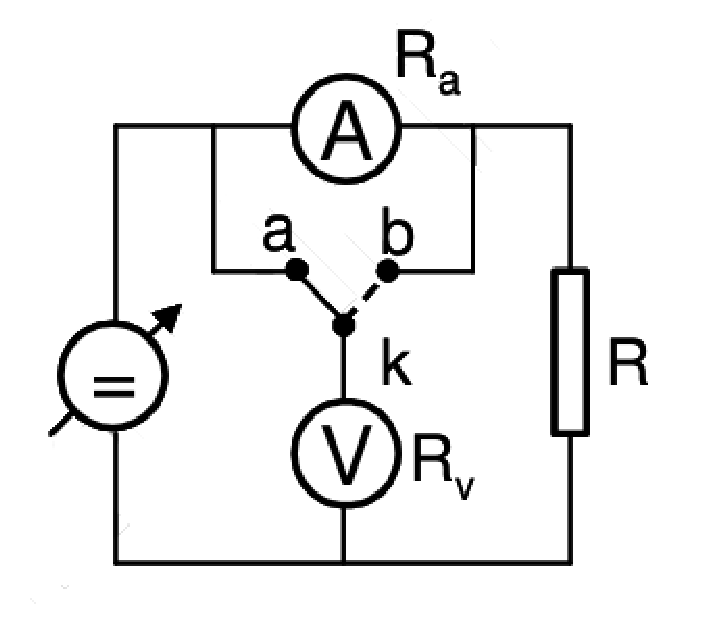
\includegraphics[scale=0.8]{sch1.eps}
\caption{Schéma pro přimou metodu.}
\end{center}
\label{sch1}
\end{figure}

\subsection{Substituční metoda měření}
Měření probíhá v zapojení dle schématu \ref{sch2}. V tomto případě naměříme proud protékající vyšetřovaným rezistorem, který následně nahradíme odporovou dekádou, 
na které nastavíme odpor tak, aby byl proud stejný jako v předchozím případě. U této metody již výsledek neovlivňuje odpor samotného ampérmetru, ale pouze 
přesnost, se kterou jsme schopni určit odpor dekády a schodu proudů.

\begin{figure}
\begin{center}
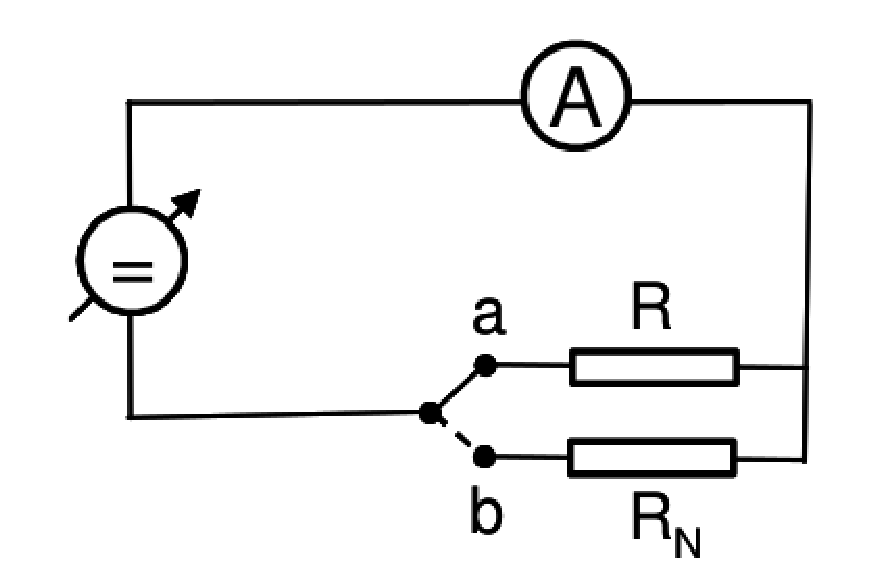
\includegraphics[scale=0.8]{sch2.eps}
\caption{Schéma pro substitční metodu.}
\label{sch2}
\end{center}
\end{figure}

\subsection{Chyby}
Při měření byly použity pouze analogové měřící přístroje. Jejich chyba je dána vztahem
\begin{eqnarray}
\sigma = k\frac{R}{100},
\end{eqnarray}
kde $k$ je třída přesnosti daného přístroje a $R$ rozsah, na kterém měříme.

Odporová dekáda má procentuální chybu odpovídající řádu odporu, který používáme. Použitá dekáda měla chybu 

Dále se vyskytuje přenos chyb. V tomto případě si vystačíme s chybou podílu a součinu, kde se relativní 
chyby veličin sčítají, a podílu a rozdílu, kdy se sčítají chyby absolutní.

\section{Měření}
\subsection{Přímá metoda}
Nejprve jsem sestavil obvod dle \ref{sch1}. Změnu proudu jsem stimuloval změnou napětí na proudu. Podle toho, kterou veličinu jsem odečital jsem měnil polohu přepínače. 
Naměřené hodnoty jsou v tabulce \ref{TUk1} spolu s dopočtenou hodnotou odporu žárovky. Výsledná závislost odporu na proudu je na obrázku \ref{g1}.

\begin{table}
$$
\begin{array}{|c|c|c|}
\hline
U/\mbox{V}& I/\mbox{mA}&    R/\Omega \\ \hline
1.000\pm 0.003&5.600\pm 0.020&179\pm1\\ \hline
2.000\pm 0.006&7.500\pm 0.020&267\pm2\\ \hline
3.00\pm 0.02&8.80\pm 0.03&341\pm3\\ \hline
4.00\pm 0.02&10.10\pm 0.03&396\pm3\\ \hline
5.00\pm 0.02&11.40\pm 0.03&439\pm3\\ \hline
6.00\pm 0.02&12.60\pm 0.03&476\pm3\\ \hline
7.00\pm 0.03&13.70\pm 0.03&511\pm3\\ \hline
8.00\pm 0.03&14.90\pm 0.03&537\pm3\\ \hline
9.00\pm 0.03&15.80\pm 0.06&570\pm4\\ \hline
10.00\pm 0.03&16.60\pm 0.06&602\pm4\\ \hline
11.00\pm 0.03&17.60\pm 0.06&625\pm4\\ \hline
12.00\pm 0.03&18.60\pm 0.06&645\pm4\\ \hline
13.00\pm 0.03&19.40\pm 0.06&670\pm4\\ \hline
14.00\pm 0.03&20.40\pm 0.06&686\pm3\\ \hline
15.00\pm 0.03&21.20\pm 0.06&708\pm3\\ \hline
16.00\pm 0.06&22.20\pm 0.06&721\pm5\\ \hline
17.00\pm 0.06&23.40\pm 0.06&726\pm4\\ \hline
18.00\pm 0.06&24.40\pm 0.06&738\pm4\\ \hline
19.00\pm 0.06&25.00\pm 0.06&760\pm4\\ \hline
20.00\pm 0.06&25.80\pm 0.06&775\pm4\\ \hline
21.00\pm 0.06&26.60\pm 0.06&789\pm4\\ \hline
22.00\pm 0.06&27.20\pm 0.06&809\pm4\\ \hline
23.00\pm 0.06&28.20\pm 0.06&816\pm4\\ \hline
24.00\pm 0.06&28.80\pm 0.06&833\pm4\\ \hline
\end{array}
$$
\caption{Výsledky měření přímou metodou bez korekcí.}
\label{TUk1}
\end{table}

\begin{figure}
% GNUPLOT: LaTeX picture with Postscript
\begingroup
  \makeatletter
  \providecommand\color[2][]{%
    \GenericError{(gnuplot) \space\space\space\@spaces}{%
      Package color not loaded in conjunction with
      terminal option `colourtext'%
    }{See the gnuplot documentation for explanation.%
    }{Either use 'blacktext' in gnuplot or load the package
      color.sty in LaTeX.}%
    \renewcommand\color[2][]{}%
  }%
  \providecommand\includegraphics[2][]{%
    \GenericError{(gnuplot) \space\space\space\@spaces}{%
      Package graphicx or graphics not loaded%
    }{See the gnuplot documentation for explanation.%
    }{The gnuplot epslatex terminal needs graphicx.sty or graphics.sty.}%
    \renewcommand\includegraphics[2][]{}%
  }%
  \providecommand\rotatebox[2]{#2}%
  \@ifundefined{ifGPcolor}{%
    \newif\ifGPcolor
    \GPcolorfalse
  }{}%
  \@ifundefined{ifGPblacktext}{%
    \newif\ifGPblacktext
    \GPblacktexttrue
  }{}%
  % define a \g@addto@macro without @ in the name:
  \let\gplgaddtomacro\g@addto@macro
  % define empty templates for all commands taking text:
  \gdef\gplbacktext{}%
  \gdef\gplfronttext{}%
  \makeatother
  \ifGPblacktext
    % no textcolor at all
    \def\colorrgb#1{}%
    \def\colorgray#1{}%
  \else
    % gray or color?
    \ifGPcolor
      \def\colorrgb#1{\color[rgb]{#1}}%
      \def\colorgray#1{\color[gray]{#1}}%
      \expandafter\def\csname LTw\endcsname{\color{white}}%
      \expandafter\def\csname LTb\endcsname{\color{black}}%
      \expandafter\def\csname LTa\endcsname{\color{black}}%
      \expandafter\def\csname LT0\endcsname{\color[rgb]{1,0,0}}%
      \expandafter\def\csname LT1\endcsname{\color[rgb]{0,1,0}}%
      \expandafter\def\csname LT2\endcsname{\color[rgb]{0,0,1}}%
      \expandafter\def\csname LT3\endcsname{\color[rgb]{1,0,1}}%
      \expandafter\def\csname LT4\endcsname{\color[rgb]{0,1,1}}%
      \expandafter\def\csname LT5\endcsname{\color[rgb]{1,1,0}}%
      \expandafter\def\csname LT6\endcsname{\color[rgb]{0,0,0}}%
      \expandafter\def\csname LT7\endcsname{\color[rgb]{1,0.3,0}}%
      \expandafter\def\csname LT8\endcsname{\color[rgb]{0.5,0.5,0.5}}%
    \else
      % gray
      \def\colorrgb#1{\color{black}}%
      \def\colorgray#1{\color[gray]{#1}}%
      \expandafter\def\csname LTw\endcsname{\color{white}}%
      \expandafter\def\csname LTb\endcsname{\color{black}}%
      \expandafter\def\csname LTa\endcsname{\color{black}}%
      \expandafter\def\csname LT0\endcsname{\color{black}}%
      \expandafter\def\csname LT1\endcsname{\color{black}}%
      \expandafter\def\csname LT2\endcsname{\color{black}}%
      \expandafter\def\csname LT3\endcsname{\color{black}}%
      \expandafter\def\csname LT4\endcsname{\color{black}}%
      \expandafter\def\csname LT5\endcsname{\color{black}}%
      \expandafter\def\csname LT6\endcsname{\color{black}}%
      \expandafter\def\csname LT7\endcsname{\color{black}}%
      \expandafter\def\csname LT8\endcsname{\color{black}}%
    \fi
  \fi
  \setlength{\unitlength}{0.0500bp}%
  \begin{picture}(7200.00,5040.00)%
    \gplgaddtomacro\gplbacktext{%
      \csname LTb\endcsname%
      \put(1210,704){\makebox(0,0)[r]{\strut{} 700}}%
      \put(1210,1074){\makebox(0,0)[r]{\strut{} 800}}%
      \put(1210,1444){\makebox(0,0)[r]{\strut{} 900}}%
      \put(1210,1814){\makebox(0,0)[r]{\strut{} 1000}}%
      \put(1210,2184){\makebox(0,0)[r]{\strut{} 1100}}%
      \put(1210,2554){\makebox(0,0)[r]{\strut{} 1200}}%
      \put(1210,2925){\makebox(0,0)[r]{\strut{} 1300}}%
      \put(1210,3295){\makebox(0,0)[r]{\strut{} 1400}}%
      \put(1210,3665){\makebox(0,0)[r]{\strut{} 1500}}%
      \put(1210,4035){\makebox(0,0)[r]{\strut{} 1600}}%
      \put(1210,4405){\makebox(0,0)[r]{\strut{} 1700}}%
      \put(1210,4775){\makebox(0,0)[r]{\strut{} 1800}}%
      \put(1342,484){\makebox(0,0){\strut{} 0}}%
      \put(2263,484){\makebox(0,0){\strut{} 0.5}}%
      \put(3184,484){\makebox(0,0){\strut{} 1}}%
      \put(4105,484){\makebox(0,0){\strut{} 1.5}}%
      \put(5027,484){\makebox(0,0){\strut{} 2}}%
      \put(5948,484){\makebox(0,0){\strut{} 2.5}}%
      \put(6869,484){\makebox(0,0){\strut{} 3}}%
      \put(308,2739){\rotatebox{-270}{\makebox(0,0){\strut{}$h$/keV$\cdot$m$^{-1}$}}}%
      \put(4105,154){\makebox(0,0){\strut{}$x$/cm}}%
    }%
    \gplgaddtomacro\gplfronttext{%
    }%
    \gplbacktext
    \put(0,0){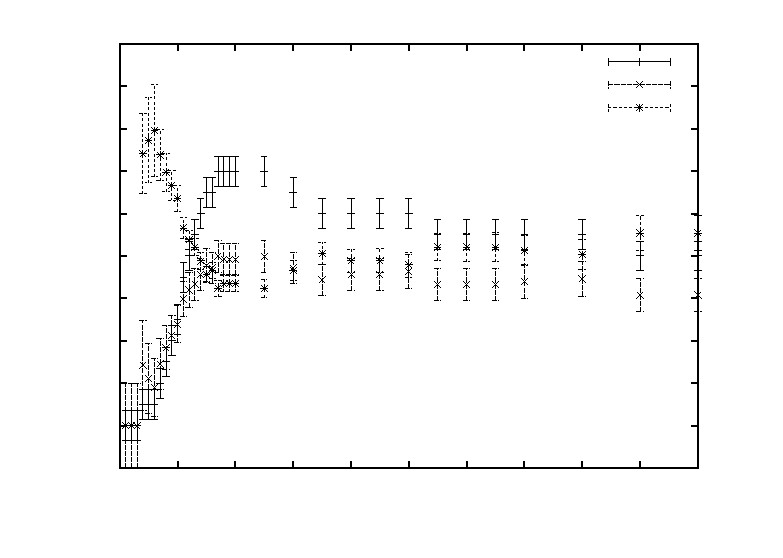
\includegraphics{g1}}%
    \gplfronttext
  \end{picture}%
\endgroup

\caption{Graf závislosti odporu na proudu měřený přímou metodou.}
\label{g1}
\end{figure}

\subsection{Odpory měřících přístrojů}
Následně jsem sestavil obvod dle \ref{sch2}, kde jsem místo rezistoru postupně zapojil přístroje použité k měření v úkolu 1. Dle postupu jsem stanovil jejich odpor v závislosti 
na rozsahu. Odpory voltmetru je v tabulce \ref{TV} a miliampérmetru v \ref{TmA}. Tyto hodnoty jsem použil ke korekci hodnot v úkolu 1. Výsledkem je tabulka \ref{TUk2}. Pro 
názornost jsem nové hodnoty vynesl s původními do stejného grafu (tedy grafu \ref{g1}) a oboje hodnoty proložil obecným polynomem.

\begin{table}
$$
\begin{array}{|c|c|}
\hline
\mbox{Rozsah/V}&  R_v/\Omega \\ \hline
30& 15000\pm20 \\ \hline
15& 7500\pm8 \\ \hline
7.5&    3725\pm4 \\ \hline
3&  1500\pm2 \\ \hline
1.5&    750\pm0.8 \\ \hline
\end{array}
$$
\caption{Odpor voltmetru v závislosti na rozsahu.}
\label{TV}
\end{table}

\begin{table}
$$
\begin{array}{|c|c|}
\hline
\mbox{Rozsah/mA}&  R_v/\Omega \\ \hline
30& 9.400\pm0.009 \\ \hline
15& 20\pm0.02 \\ \hline
7.5& 38\pm 0.04 \\ \hline
\end{array}
$$
\caption{Odpor miliapérmetru v závislosti na rozsahu}
\label{TmA}
\end{table}

\begin{table}
$$
\begin{array}{|c|c|}
\hline
I/\mbox{mA}&    R/\Omega \\ \hline
4.52\pm 0.03&217\pm 1\\ \hline
6.37\pm 0.04&305\pm 1\\ \hline
7.17\pm 0.08&379\pm 2\\ \hline
9.13\pm 0.08&434\pm 2\\ \hline
10.20\pm 0.08&477\pm 2\\ \hline
11.17\pm 0.08&514\pm 2\\ \hline
12.05\pm 0.09&549\pm 2\\ \hline
13.90\pm 0.09&557\pm 2\\ \hline
14.7\pm 0.1&590\pm 3\\ \hline
15.4\pm 0.1&622\pm 3\\ \hline
16.2\pm 0.1&645\pm 3\\ \hline
17.1\pm 0.1&665\pm 3\\ \hline
17.8\pm 0.1&690\pm 3\\ \hline
18.7\pm 0.1&706\pm 3\\ \hline
19.4\pm 0.1&728\pm 3\\ \hline
21.2\pm 0.2&730\pm 3\\ \hline
22.3\pm 0.2&736\pm 3\\ \hline
23.3\pm 0.2&747\pm 3\\ \hline
23.8\pm 0.2&769\pm 3\\ \hline
24.5\pm 0.2&785\pm 3\\ \hline
25.3\pm 0.2&799\pm 3\\ \hline
25.8\pm 0.2&818\pm 3\\ \hline
26.7\pm 0.2&825\pm 3\\ \hline
27.3\pm 0.2&843\pm 3\\ \hline
\end{array}
$$
\caption{Výsledky měření přímou metodou s použitím korekcí.}
\label{TUk2}
\end{table}



\subsection{Substituční metoda}
R ve schématu \ref{sch2} jsem nahradil žárovkou a následně změřil její odpor v závislosti na proudu. Hodnoty jsou v tabulce \ref{TUk3} a na obrázku \ref{g2}, kde jsou opět 
pro názornost proloženy obecným polynomem. Z tohoto grafu jsem též extrapoloval velikost 
odporu žárovky pro nulpvý proud, která byla
\begin{eqnarray}
R_0=(118.8\pm0.8)\Omega
\end{eqnarray}

\begin{table}
$$
\begin{array}{|c|c|}
\hline
I/\mbox{mA}&    R/\Omega \\ \hline
0.240\pm 0.003&118.0\pm 0.1\\ \hline
0.640\pm 0.003&118.0\pm 0.1\\ \hline
0.860\pm 0.003&118.0\pm 0.1\\ \hline
1.000\pm 0.003&118.0\pm 0.1\\ \hline
1.960\pm 0.003&122.0\pm 0.1\\ \hline
3.000\pm 0.003&130.0\pm 0.1\\ \hline
4.00\pm 0.02&143.0\pm 0.1\\ \hline
5.00\pm 0.02&164.0\pm 0.2\\ \hline
6.00\pm 0.02&200.0\pm 0.2\\ \hline
7.05\pm 0.02&254.0\pm 0.3\\ \hline
8.10\pm 0.03&306.0\pm 0.3\\ \hline
9.10\pm 0.03&352.0\pm 0.4\\ \hline
10.00\pm 0.03&388.0\pm 0.4\\ \hline
11.00\pm 0.03&428.0\pm 0.4\\ \hline
12.10\pm 0.03&458.0\pm 0.5\\ \hline
13.20\pm 0.03&496.0\pm 0.5\\ \hline
14.00\pm 0.03&521.0\pm 0.5\\ \hline
15.00\pm 0.06&548.0\pm 0.5\\ \hline
16.00\pm 0.06&580.0\pm 0.6\\ \hline
17.00\pm 0.06&610.0\pm 0.6\\ \hline
18.00\pm 0.06&636.0\pm 0.6\\ \hline
19.00\pm 0.06&656.0\pm 0.7\\ \hline
20.00\pm 0.06&680.0\pm 0.7\\ \hline
21.00\pm 0.06&691.0\pm 0.7\\ \hline
\end{array}
$$
\caption{Výsledky měření substituční metodou.}
\label{TUk3}
\end{table}

\begin{figure}
% GNUPLOT: LaTeX picture with Postscript
\begingroup
  \makeatletter
  \providecommand\color[2][]{%
    \GenericError{(gnuplot) \space\space\space\@spaces}{%
      Package color not loaded in conjunction with
      terminal option `colourtext'%
    }{See the gnuplot documentation for explanation.%
    }{Either use 'blacktext' in gnuplot or load the package
      color.sty in LaTeX.}%
    \renewcommand\color[2][]{}%
  }%
  \providecommand\includegraphics[2][]{%
    \GenericError{(gnuplot) \space\space\space\@spaces}{%
      Package graphicx or graphics not loaded%
    }{See the gnuplot documentation for explanation.%
    }{The gnuplot epslatex terminal needs graphicx.sty or graphics.sty.}%
    \renewcommand\includegraphics[2][]{}%
  }%
  \providecommand\rotatebox[2]{#2}%
  \@ifundefined{ifGPcolor}{%
    \newif\ifGPcolor
    \GPcolorfalse
  }{}%
  \@ifundefined{ifGPblacktext}{%
    \newif\ifGPblacktext
    \GPblacktexttrue
  }{}%
  % define a \g@addto@macro without @ in the name:
  \let\gplgaddtomacro\g@addto@macro
  % define empty templates for all commands taking text:
  \gdef\gplbacktext{}%
  \gdef\gplfronttext{}%
  \makeatother
  \ifGPblacktext
    % no textcolor at all
    \def\colorrgb#1{}%
    \def\colorgray#1{}%
  \else
    % gray or color?
    \ifGPcolor
      \def\colorrgb#1{\color[rgb]{#1}}%
      \def\colorgray#1{\color[gray]{#1}}%
      \expandafter\def\csname LTw\endcsname{\color{white}}%
      \expandafter\def\csname LTb\endcsname{\color{black}}%
      \expandafter\def\csname LTa\endcsname{\color{black}}%
      \expandafter\def\csname LT0\endcsname{\color[rgb]{1,0,0}}%
      \expandafter\def\csname LT1\endcsname{\color[rgb]{0,1,0}}%
      \expandafter\def\csname LT2\endcsname{\color[rgb]{0,0,1}}%
      \expandafter\def\csname LT3\endcsname{\color[rgb]{1,0,1}}%
      \expandafter\def\csname LT4\endcsname{\color[rgb]{0,1,1}}%
      \expandafter\def\csname LT5\endcsname{\color[rgb]{1,1,0}}%
      \expandafter\def\csname LT6\endcsname{\color[rgb]{0,0,0}}%
      \expandafter\def\csname LT7\endcsname{\color[rgb]{1,0.3,0}}%
      \expandafter\def\csname LT8\endcsname{\color[rgb]{0.5,0.5,0.5}}%
    \else
      % gray
      \def\colorrgb#1{\color{black}}%
      \def\colorgray#1{\color[gray]{#1}}%
      \expandafter\def\csname LTw\endcsname{\color{white}}%
      \expandafter\def\csname LTb\endcsname{\color{black}}%
      \expandafter\def\csname LTa\endcsname{\color{black}}%
      \expandafter\def\csname LT0\endcsname{\color{black}}%
      \expandafter\def\csname LT1\endcsname{\color{black}}%
      \expandafter\def\csname LT2\endcsname{\color{black}}%
      \expandafter\def\csname LT3\endcsname{\color{black}}%
      \expandafter\def\csname LT4\endcsname{\color{black}}%
      \expandafter\def\csname LT5\endcsname{\color{black}}%
      \expandafter\def\csname LT6\endcsname{\color{black}}%
      \expandafter\def\csname LT7\endcsname{\color{black}}%
      \expandafter\def\csname LT8\endcsname{\color{black}}%
    \fi
  \fi
  \setlength{\unitlength}{0.0500bp}%
  \begin{picture}(7200.00,5040.00)%
    \gplgaddtomacro\gplbacktext{%
      \csname LTb\endcsname%
      \put(814,704){\makebox(0,0)[r]{\strut{} 0}}%
      \put(814,1213){\makebox(0,0)[r]{\strut{} 1}}%
      \put(814,1722){\makebox(0,0)[r]{\strut{} 2}}%
      \put(814,2231){\makebox(0,0)[r]{\strut{} 3}}%
      \put(814,2740){\makebox(0,0)[r]{\strut{} 4}}%
      \put(814,3248){\makebox(0,0)[r]{\strut{} 5}}%
      \put(814,3757){\makebox(0,0)[r]{\strut{} 6}}%
      \put(814,4266){\makebox(0,0)[r]{\strut{} 7}}%
      \put(814,4775){\makebox(0,0)[r]{\strut{} 8}}%
      \put(946,484){\makebox(0,0){\strut{} 0}}%
      \put(1404,484){\makebox(0,0){\strut{} 0.1}}%
      \put(1863,484){\makebox(0,0){\strut{} 0.2}}%
      \put(2321,484){\makebox(0,0){\strut{} 0.3}}%
      \put(2780,484){\makebox(0,0){\strut{} 0.4}}%
      \put(3238,484){\makebox(0,0){\strut{} 0.5}}%
      \put(3697,484){\makebox(0,0){\strut{} 0.6}}%
      \put(4155,484){\makebox(0,0){\strut{} 0.7}}%
      \put(4614,484){\makebox(0,0){\strut{} 0.8}}%
      \put(5072,484){\makebox(0,0){\strut{} 0.9}}%
      \put(5531,484){\makebox(0,0){\strut{} 1}}%
      \put(5989,484){\makebox(0,0){\strut{} 1.1}}%
      \put(6121,1043){\makebox(0,0)[l]{\strut{} 56}}%
      \put(6121,1722){\makebox(0,0)[l]{\strut{} 58}}%
      \put(6121,2400){\makebox(0,0)[l]{\strut{} 60}}%
      \put(6121,3079){\makebox(0,0)[l]{\strut{} 62}}%
      \put(6121,3757){\makebox(0,0)[l]{\strut{} 64}}%
      \put(6121,4436){\makebox(0,0)[l]{\strut{} 66}}%
      \put(308,2739){\rotatebox{-270}{\makebox(0,0){\strut{}$C/\mu$F}}}%
      \put(6758,2739){\rotatebox{-270}{\makebox(0,0){\strut{}$\tau/$s}}}%
      \put(3467,154){\makebox(0,0){\strut{}$I/$mA}}%
    }%
    \gplgaddtomacro\gplfronttext{%
      \csname LTb\endcsname%
      \put(5002,1317){\makebox(0,0)[r]{\strut{}$C$}}%
      \csname LTb\endcsname%
      \put(5002,1097){\makebox(0,0)[r]{\strut{}$7.72\cdot10^{-3}\{I\}$}}%
      \csname LTb\endcsname%
      \put(5002,877){\makebox(0,0)[r]{\strut{}$\tau$}}%
    }%
    \gplbacktext
    \put(0,0){\includegraphics{g2}}%
    \gplfronttext
  \end{picture}%
\endgroup

\caption{Graf závislosti odporu na proudu měřený substituční metodou.}
\label{g2}
\end{figure}

Nakonec jsem vynesl do grafu společně zavislost odporu na porudu měřenou přimou metodou s korekturami a metodou substituční. Výsledek je obrázek \ref{g3}.

\begin{figure}
% GNUPLOT: LaTeX picture with Postscript
\begingroup
  \makeatletter
  \providecommand\color[2][]{%
    \GenericError{(gnuplot) \space\space\space\@spaces}{%
      Package color not loaded in conjunction with
      terminal option `colourtext'%
    }{See the gnuplot documentation for explanation.%
    }{Either use 'blacktext' in gnuplot or load the package
      color.sty in LaTeX.}%
    \renewcommand\color[2][]{}%
  }%
  \providecommand\includegraphics[2][]{%
    \GenericError{(gnuplot) \space\space\space\@spaces}{%
      Package graphicx or graphics not loaded%
    }{See the gnuplot documentation for explanation.%
    }{The gnuplot epslatex terminal needs graphicx.sty or graphics.sty.}%
    \renewcommand\includegraphics[2][]{}%
  }%
  \providecommand\rotatebox[2]{#2}%
  \@ifundefined{ifGPcolor}{%
    \newif\ifGPcolor
    \GPcolorfalse
  }{}%
  \@ifundefined{ifGPblacktext}{%
    \newif\ifGPblacktext
    \GPblacktexttrue
  }{}%
  % define a \g@addto@macro without @ in the name:
  \let\gplgaddtomacro\g@addto@macro
  % define empty templates for all commands taking text:
  \gdef\gplbacktext{}%
  \gdef\gplfronttext{}%
  \makeatother
  \ifGPblacktext
    % no textcolor at all
    \def\colorrgb#1{}%
    \def\colorgray#1{}%
  \else
    % gray or color?
    \ifGPcolor
      \def\colorrgb#1{\color[rgb]{#1}}%
      \def\colorgray#1{\color[gray]{#1}}%
      \expandafter\def\csname LTw\endcsname{\color{white}}%
      \expandafter\def\csname LTb\endcsname{\color{black}}%
      \expandafter\def\csname LTa\endcsname{\color{black}}%
      \expandafter\def\csname LT0\endcsname{\color[rgb]{1,0,0}}%
      \expandafter\def\csname LT1\endcsname{\color[rgb]{0,1,0}}%
      \expandafter\def\csname LT2\endcsname{\color[rgb]{0,0,1}}%
      \expandafter\def\csname LT3\endcsname{\color[rgb]{1,0,1}}%
      \expandafter\def\csname LT4\endcsname{\color[rgb]{0,1,1}}%
      \expandafter\def\csname LT5\endcsname{\color[rgb]{1,1,0}}%
      \expandafter\def\csname LT6\endcsname{\color[rgb]{0,0,0}}%
      \expandafter\def\csname LT7\endcsname{\color[rgb]{1,0.3,0}}%
      \expandafter\def\csname LT8\endcsname{\color[rgb]{0.5,0.5,0.5}}%
    \else
      % gray
      \def\colorrgb#1{\color{black}}%
      \def\colorgray#1{\color[gray]{#1}}%
      \expandafter\def\csname LTw\endcsname{\color{white}}%
      \expandafter\def\csname LTb\endcsname{\color{black}}%
      \expandafter\def\csname LTa\endcsname{\color{black}}%
      \expandafter\def\csname LT0\endcsname{\color{black}}%
      \expandafter\def\csname LT1\endcsname{\color{black}}%
      \expandafter\def\csname LT2\endcsname{\color{black}}%
      \expandafter\def\csname LT3\endcsname{\color{black}}%
      \expandafter\def\csname LT4\endcsname{\color{black}}%
      \expandafter\def\csname LT5\endcsname{\color{black}}%
      \expandafter\def\csname LT6\endcsname{\color{black}}%
      \expandafter\def\csname LT7\endcsname{\color{black}}%
      \expandafter\def\csname LT8\endcsname{\color{black}}%
    \fi
  \fi
  \setlength{\unitlength}{0.0500bp}%
  \begin{picture}(7200.00,5040.00)%
    \gplgaddtomacro\gplbacktext{%
      \csname LTb\endcsname%
      \put(1210,704){\makebox(0,0)[r]{\strut{} 0}}%
      \put(1210,1382){\makebox(0,0)[r]{\strut{} 500}}%
      \put(1210,2061){\makebox(0,0)[r]{\strut{} 1000}}%
      \put(1210,2739){\makebox(0,0)[r]{\strut{} 1500}}%
      \put(1210,3418){\makebox(0,0)[r]{\strut{} 2000}}%
      \put(1210,4096){\makebox(0,0)[r]{\strut{} 2500}}%
      \put(1210,4775){\makebox(0,0)[r]{\strut{} 3000}}%
      \put(1342,484){\makebox(0,0){\strut{} 30}}%
      \put(1956,484){\makebox(0,0){\strut{} 40}}%
      \put(2570,484){\makebox(0,0){\strut{} 50}}%
      \put(3184,484){\makebox(0,0){\strut{} 60}}%
      \put(3798,484){\makebox(0,0){\strut{} 70}}%
      \put(4413,484){\makebox(0,0){\strut{} 80}}%
      \put(5027,484){\makebox(0,0){\strut{} 90}}%
      \put(5641,484){\makebox(0,0){\strut{} 100}}%
      \put(6255,484){\makebox(0,0){\strut{} 110}}%
      \put(6869,484){\makebox(0,0){\strut{} 120}}%
      \put(308,2739){\rotatebox{-270}{\makebox(0,0){\strut{}$f$/Hz}}}%
      \put(4105,154){\makebox(0,0){\strut{}$U_0$/V}}%
    }%
    \gplgaddtomacro\gplfronttext{%
    }%
    \gplbacktext
    \put(0,0){\includegraphics{g3}}%
    \gplfronttext
  \end{picture}%
\endgroup

\caption{Graf závislosti odporu na proudu měřený substituční a přímou metodou.}
\label{g3}
\end{figure}

\section{Dikuze}
Nejmenší chybu měla jednoznačně substituční metoda a to díky malé chybě odporové dekády a tomu, 
že při měření nebyl potřeba voltmetr. Ten byl totiž největším zdrojem chyby díky velikosti odporu 
uvnitř. Výsledky obou metod by však měli být až na chybu podobné, což zjevně nenastalo. Hodnoty 
se k sobě začli blížit až při větších proudech. Tato chyba je podle mě způsobena rozídlným 
ohříváním žárovky. U přímé metody totiž žárovkou tekl téměř neustále proud, zatímco u substituční 
metody žárovka chladla při hledání správného odporu na dekádě. To bylo vidět zejména při 
opětovném zapnutí proudu žárovkou, kdy ručička miliapérmetru po chvíli znatelně poklesla.

Korekce přímé metody jistě zpřesnili výsledky, protože bez nich by byl rozdíl mezi metodami ještě 
větší.

Odpor vlákna žárovky za pokojové teploty jsem mohl stanovit pouze ze substituční metody, protože 
u přímé  se mi nepodařilo stimulovat dostatečně malý proud k možné extrapolaci.

\section{Závěr}
Změřil jsem přímou metodou závislost odporu vlákna žárovku na proudu. Výsledky jsou v tabulce 
\ref{TUk1} a na obrázku \ref{g1}.\\
Změřil jsem substituční metodou odpory měřících přístrojů použitých v úkolu 1. Výsledky jsou 
v tabulkách \ref{TV} a \ref{TmA}.\\
Použil jsem odpory měřících přístrojů ke korekci hodnot z úkolu 1. Výsledky jsou v tabulce 
\ref{TUk2} a na obrázku \ref{g1}. \\
Substituční metodou jsem změřil závislost odporu vlákna na proudu. Výsledky jsou v tabulce 
\ref{TUk3} ana obrázku \ref{g2}. Dále jsem extrapoloval velikost odporu vlákna při pokojové 
teploté, která byla
\begin{eqnarray}
R_0=(118.8\pm0.8)\Omega.
\end{eqnarray}

\begin{thebibliography}{5}
	\bibitem{text} \textbf{Studijní text na praktikum II} \\http://physics.mff.cuni.cz/vyuka/zfp/txt\_202.pdf (26. 11. 2011)
    \bibitem{chyba} \emph{J. Englich}: \textbf{Zpracování výsldků fyzikálních měření} \\ LS 1999/2000
\end{thebibliography}




\end{document}

